\chapter{Analyse Approfondie des Fonctionnalités et Techniques}

\section*{Introduction}
\addcontentsline{toc}{section}{Introduction}

La plateforme est organisée en cinq couches indépendantes mais interconnectées, couvrant
l'ensemble du cycle de vie de la donnée scientifique : depuis la découverte et l'ingestion
des articles ArXiv jusqu'à la génération de réponses citées, en passant par l'indexation,
la récupération hybride et l'évaluation quantitative de la qualité. Cette architecture
en couches a été conçue pour permettre une validation indépendante de chaque étage avant
toute composition avec les étages suivants, conformément à la méthodologie de développement
adoptée tout au long du projet.

\usetikzlibrary{positioning, arrows.meta}

\section{Architecture Globale}

\begin{figure}[H]
    \centering
    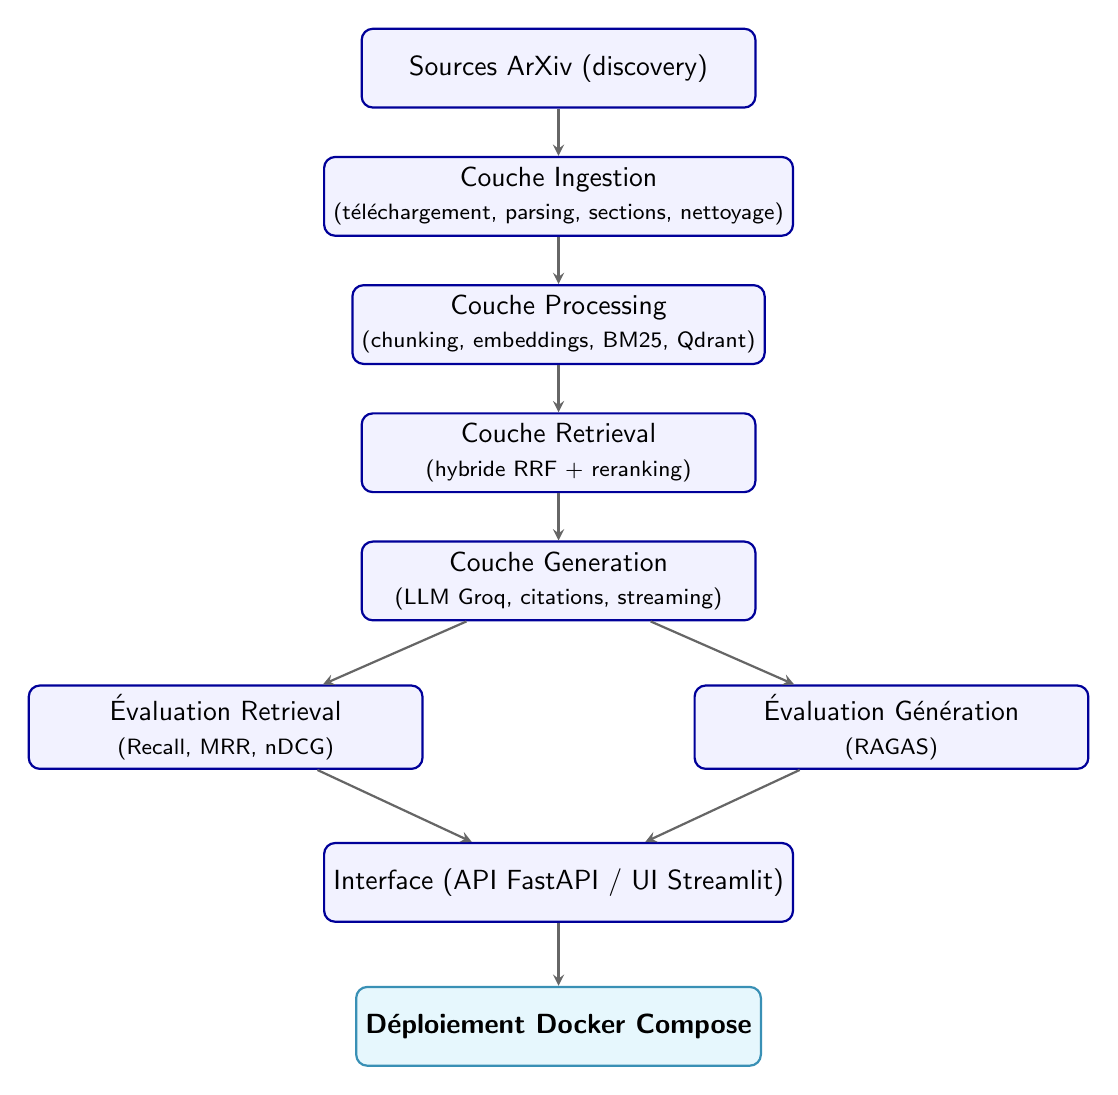
\begin{tikzpicture}[
        box/.style={
            rectangle,
            rounded corners,
            draw=blue!60!black,
            fill=blue!5,
            thick,
            minimum width=5cm,
            minimum height=1cm,
            align=center,
            font=\sffamily
        },
        dockerbox/.style={
            rectangle,
            rounded corners,
            draw=cyan!70!black,
            fill=cyan!10,
            thick,
            minimum width=5cm,
            minimum height=1cm,
            align=center,
            font=\sffamily\bfseries
        },
        arrow/.style={
            ->,
            >=stealth,
            thick,
            draw=gray!80!black
        }
    ]

    % Noeuds du pipeline
    \node[box] (A) {Sources ArXiv (discovery)};
    \node[box, below=0.6cm of A] (B) {Couche Ingestion\\ \footnotesize (téléchargement, parsing, sections, nettoyage)};
    \node[box, below=0.6cm of B] (C) {Couche Processing\\ \footnotesize (chunking, embeddings, BM25, Qdrant)};
    \node[box, below=0.6cm of C] (D) {Couche Retrieval\\ \footnotesize (hybride RRF + reranking)};
    \node[box, below=0.6cm of D] (E) {Couche Generation\\ \footnotesize (LLM Groq, citations, streaming)};

    % Embranchement évaluation
    \node[box, below left=0.8cm and -0.8cm of E] (F) {Évaluation Retrieval\\ \footnotesize (Recall, MRR, nDCG)};
    \node[box, below right=0.8cm and -0.8cm of E] (G) {Évaluation Génération\\ \footnotesize (RAGAS)};

    % Interface
    \node[box, below=2.8cm of E] (H) {Interface (API FastAPI / UI Streamlit)};

    % Étape finale : déploiement
    \node[dockerbox, below=0.8cm of H] (I) {Déploiement Docker Compose};

    % Tracé des flèches
    \draw[arrow] (A) -- (B);
    \draw[arrow] (B) -- (C);
    \draw[arrow] (C) -- (D);
    \draw[arrow] (D) -- (E);
    \draw[arrow] (E) -- (F);
    \draw[arrow] (E) -- (G);
    \draw[arrow] (F) -- (H);
    \draw[arrow] (G) -- (H);
    \draw[arrow] (H) -- (I);

    \end{tikzpicture}
    \caption{Architecture en couches du pipeline RAG, de l'ingestion au déploiement}
    \label{fig:pipeline_rag}
\end{figure}

% ─── 3.1 ─────────────────────────────────────────────────────────────────────
\section{Spécifications fonctionnelles}

\subsection{Couche d'ingestion}

\subsubsection{Module de découverte et de collecte des articles}

Ce module assure la découverte et le rapatriement fiable des articles scientifiques
depuis ArXiv. L'utilisateur soumet une requête thématique (par exemple
\textit{« retrieval augmented generation »}) et le système interroge successivement
plusieurs fournisseurs de découverte selon une stratégie de repli en cascade : un
serveur MCP alphaXiv, éventuellement assisté d'un planificateur de requêtes basé sur
Groq, puis en dernier recours l'API ArXiv officielle, garantie déterministe et
toujours disponible.

Un mécanisme de normalisation harmonise les réponses hétérogènes des différents
fournisseurs en un schéma commun (\texttt{Paper}), déduplique les résultats sur la
base de l'identifiant ArXiv, du DOI et du titre normalisé, puis les classe par
pertinence en combinant un score sémantique et le nombre de citations lorsqu'il est
disponible.

Le téléchargement des PDF s'appuie ensuite sur un registre SQLite qui évite les
téléchargements redondants, gère les échecs réseau transitoires par nouvelles
tentatives, et ne promeut un fichier que si la validité du PDF a été vérifiée
(écriture atomique via fichier temporaire \texttt{.part}).

\begin{encadre}[Bibliothèques utilisées]
\begin{itemize}
  \item \textbf{arxiv} — client Python pour l'API de recherche ArXiv.
  \item \textbf{httpx} — client HTTP asynchrone pour le téléchargement des PDF et les
        appels aux fournisseurs de découverte enrichie.
  \item \textbf{Model Context Protocol (MCP)} — intégration du serveur alphaXiv via un
        sous-processus JSON-RPC.
  \item \textbf{SQLite} — registre persistant de l'état d'ingestion (téléchargé, indexé,
        en échec).
\end{itemize}
\end{encadre}

\subsubsection{Module d'extraction et de structuration}

Ce module transforme un PDF brut en document structuré et exploitable pour
l'indexation. L'extraction du texte s'effectue page par page via PyMuPDF, préservant
la pagination d'origine. Un détecteur de sections, fondé sur des heuristiques
d'en-têtes (expressions régulières et règles de forme), segmente ensuite le texte en
sections canoniques de l'article scientifique : résumé, introduction, travaux
connexes, méthode, expérimentations, conclusion et références.

L'extracteur de métadonnées produit un enregistrement homogène (titre, auteurs,
année, catégorie ArXiv, DOI) quelle que soit la source de découverte d'origine, tandis
que l'extracteur de citations isole la liste des références et tente d'y repérer les
identifiants ArXiv et DOI cités par l'article.

\paragraph{Nettoyage des données}

Le nettoyage, réalisé par le module \texttt{data\_cleaner}, corrige les artefacts
typiques de l'extraction PDF : recomposition des mots coupés en fin de ligne,
suppression des numéros de page isolés, retrait des commandes LaTeX résiduelles et
des lignes répétées (en-têtes et pieds de page récurrents), puis normalisation des
espaces et des sauts de ligne. Cette étape est indispensable avant le découpage en
segments, car des artefacts non corrigés dégradent directement la qualité des
embeddings ultérieurs.

\begin{encadre}[Bibliothèques utilisées]
\begin{itemize}
  \item \textbf{PyMuPDF (fitz)} — extraction du texte page par page.
  \item \textbf{re} — détection des en-têtes de section et nettoyage par motifs.
\end{itemize}
\end{encadre}

% ─── 3.2 ─────────────────────────────────────────────────────────────────────
\subsection{Couche de traitement (processing)}

\paragraph{Résumé exécutif}

La couche de traitement transforme les documents sectionnés et nettoyés en unités
indexables. Elle réalise trois opérations principales : le découpage du texte en
segments (\emph{chunks}), la génération de leurs représentations vectorielles
(\emph{embeddings}) et leur indexation selon deux approches complémentaires, dense et
lexicale. Les segments obtenus sont ensuite prêts à être utilisés par le système de
récupération.

\subsubsection{Découpage en segments (chunking)}

Le découpage privilégie une stratégie \emph{section-aware} plutôt qu'une fenêtre fixe
arbitraire. Chaque section détectée constitue une unité de base. Lorsqu'une section
dépasse la taille maximale de tokens configurée, elle est subdivisée à l'aide d'une
fenêtre glissante avec chevauchement. À l'inverse, une section trop courte est
fusionnée avec une section adjacente. Pour les documents dans lesquels aucune
structure de sections n'a pu être détectée, un découpage générique par fenêtre
glissante est utilisé comme solution de repli.

Chaque segment reçoit un identifiant déterministe dérivé de son contenu. Il conserve
également ses offsets de caractères dans le document source ainsi que l'étiquette de
sa section d'origine. Ces métadonnées assurent une traçabilité complète entre une
réponse générée et le passage précis de l'article utilisé pour la produire.

\subsubsection{Génération des embeddings}

Un \emph{embedding} est une représentation numérique dense d'un texte sous la forme
d'un vecteur. Des segments dont le sens est proche produisent généralement des
vecteurs proches dans l'espace vectoriel, même lorsqu'ils n'emploient pas exactement
les mêmes mots.

Dans l'implémentation, chaque segment est encodé par le composant
\texttt{embedder} à l'aide du modèle \texttt{sentence-transformers}
\texttt{all-MiniLM-L6-v2}. Ce modèle génère un vecteur de 384 dimensions pour chaque
segment. Il est chargé une seule fois au début de la session, puis réutilisé pour
l'ensemble du corpus afin d'éviter des chargements répétés et de réduire le temps de
traitement.

\subsubsection{Indexation dense avec Qdrant}

L'indexation dense permet de retrouver des passages selon leur proximité sémantique.
Elle est particulièrement utile lorsqu'une requête et un segment expriment une même
idée avec des formulations différentes.

Les embeddings des segments sont stockés dans la base vectorielle \texttt{Qdrant},
accompagnés de leur texte et de leurs métadonnées. Lors d'une recherche, la requête
est encodée avec le même modèle, puis son vecteur est comparé aux vecteurs enregistrés
en utilisant la similarité cosinus. Qdrant retourne ainsi les segments dont le sens
est le plus proche de celui de la requête.

\subsubsection{Indexation lexicale avec BM25}

L'indexation lexicale recherche les segments à partir des mots effectivement présents
dans le texte. Elle complète la recherche dense en favorisant les correspondances
exactes, notamment pour les noms de modèles, les acronymes, les termes techniques et
les titres d'articles.

Dans l'implémentation, les segments sont tokenisés puis transmis à
\texttt{BM25Okapi}, fourni par la bibliothèque \texttt{rank\_bm25}. Pour chaque
requête, BM25 attribue un score aux segments selon la présence et l'importance des
termes recherchés dans le corpus. L'index construit est sérialisé sur disque afin de
pouvoir être rechargé lors des sessions suivantes sans devoir être reconstruit.

Les index dense et lexical sont donc complémentaires : Qdrant recherche principalement
la proximité de sens, tandis que BM25 privilégie la correspondance des termes. Leur
utilisation conjointe améliore la couverture et la précision de la récupération.

\begin{encadre}[Bibliothèques utilisées]
\begin{itemize}
  \item \textbf{sentence-transformers} — génération des embeddings denses avec le
        modèle \texttt{all-MiniLM-L6-v2}.
  \item \textbf{Qdrant} — stockage des vecteurs et recherche sémantique par similarité
        cosinus.
  \item \textbf{rank\_bm25} — construction et interrogation de l'index lexical
        \texttt{BM25Okapi}.
\end{itemize}
\end{encadre}

% ─── 3.3 ─────────────────────────────────────────────────────────────────────
\subsection{Couche de récupération (retrieval)}

\paragraph{Résumé exécutif}

La couche de récupération transforme une requête utilisateur en un ensemble restreint
de segments pertinents. Elle combine une recherche sémantique et une recherche
lexicale, fusionne leurs résultats, puis affine leur classement à l'aide d'un modèle
de reclassement plus précis. Une étape optionnelle de diversification permet enfin de
limiter la redondance entre les passages sélectionnés.

\subsubsection{Recherche hybride}

La requête est d'abord nettoyée, puis transmise simultanément aux deux systèmes de
recherche. La recherche dense compare son embedding à ceux des segments stockés dans
Qdrant à l'aide de la similarité cosinus. En parallèle, la recherche lexicale BM25
identifie les segments contenant les termes les plus significatifs de la requête.

Ces deux approches sont complémentaires : la recherche dense reconnaît les proximités
de sens, tandis que BM25 privilégie les correspondances lexicales exactes. Elles
produisent toutefois des scores de nature et d'échelle différentes. Leurs résultats
sont donc combinés avec la méthode \emph{Reciprocal Rank Fusion} (RRF), qui utilise la
position des documents dans chaque classement plutôt que leurs scores bruts :

\[
  \operatorname{score}_{\mathrm{RRF}}(d)
  =
  \sum_{i\,:\,d \in L_i}
  \frac{1}{k + \operatorname{rang}_{i}(d)},
  \qquad k = 60
\]

où \(L_i\) représente un classement produit par un moteur de recherche et
\(\operatorname{rang}_{i}(d)\) la position du segment \(d\) dans ce classement. Un
segment absent d'un classement ne contribue pas à la somme.

Cette méthode ne nécessite aucune normalisation préalable des scores. Elle favorise
les segments bien positionnés dans plusieurs classements, tout en conservant les
résultats particulièrement pertinents trouvés par une seule méthode.

\subsubsection{Reclassement des candidats}

La fusion RRF fournit rapidement une première liste de candidats. Les mieux classés
sont ensuite réévalués par le \emph{cross-encoder}
\texttt{cross-encoder/ms-marco-MiniLM-L-6-v2}.

Contrairement au modèle d'embedding, qui encode séparément la requête et les segments,
le \emph{cross-encoder} analyse conjointement chaque paire composée de la requête et
d'un segment. Il produit ainsi un score de pertinence plus précis, mais son coût de
calcul est plus élevé. Pour cette raison, il est uniquement appliqué au nombre limité
de candidats présélectionnés par la recherche hybride.

Les candidats sont finalement triés selon les scores produits par le
\emph{cross-encoder}, et les mieux classés sont transmis aux étapes suivantes du
pipeline.

\subsubsection{Diversification avec MMR}

Une étape optionnelle de \emph{Maximal Marginal Relevance} (MMR) peut être appliquée
après le reclassement. Elle sélectionne progressivement les segments en recherchant
un compromis entre deux objectifs : leur pertinence par rapport à la requête et leur
différence par rapport aux segments déjà retenus.

Cette diversification évite que le contexte final soit composé de plusieurs passages
presque identiques, par exemple lorsque différentes sections ou plusieurs segments
chevauchants d'un même article présentent la même information. Elle permet ainsi
d'exploiter plus efficacement l'espace de contexte disponible.

\subsubsection{Enrichissement déclenché par la récupération}

Lorsque les résultats disponibles ne satisfont pas les critères de pertinence
configurés, le système peut déclencher automatiquement une ingestion ciblée de
nouveaux articles. Cette décision peut notamment dépendre du nombre de résultats
obtenus, du meilleur score de pertinence ou d'une fonction de seuil personnalisée.

Les nouveaux documents sont alors collectés, nettoyés, segmentés et encodés. Leurs
vecteurs et métadonnées sont ajoutés à Qdrant, tandis que l'index BM25 est reconstruit
à partir de l'ensemble des segments enregistrés afin d'intégrer le corpus enrichi. La
requête initiale est ensuite relancée sur les index mis à jour.

Ce mécanisme permet au corpus de s'étendre à la demande lorsque les connaissances
locales sont insuffisantes, tout en conservant un seul pipeline de récupération.

\begin{encadre}[Bibliothèques utilisées]
\begin{itemize}
  \item \textbf{Qdrant Client} — recherche vectorielle par similarité cosinus et
        application éventuelle de filtres sur les métadonnées.
  \item \textbf{sentence-transformers} — encodage dense des requêtes et reclassement
        des candidats avec la classe \texttt{CrossEncoder}.
  \item \textbf{rank\_bm25} — recherche lexicale avec l'algorithme
        \texttt{BM25Okapi}.
\end{itemize}
\end{encadre}

% ─── 3.4 ─────────────────────────────────────────────────────────────────────
\subsection{Analyse et évaluation de la récupération}

\paragraph{Résumé exécutif}

La plateforme évalue séparément la récupération et la génération. Cette séparation
permet de déterminer si une réponse incorrecte provient de l'absence des passages
pertinents dans le contexte récupéré ou d'une mauvaise exploitation de ces passages
par le modèle de génération.

L'évaluation de la récupération compare plusieurs configurations du pipeline selon
leur capacité à retrouver et à classer les segments de référence, tout en mesurant
leur coût en temps d'exécution.

\subsubsection{Jeu de données de référence}

L'évaluation repose sur un ensemble de questions associées à des jugements de
pertinence. Les annotations peuvent être définies au niveau de l'article ou, de
manière plus précise, au niveau du segment. Lorsque des segments de référence ont été
validés manuellement, l'évaluation utilise directement leurs identifiants. Dans le
cas contraire, elle applique explicitement un repli vers les identifiants des
articles pertinents.

Une interface en ligne de commande permet de réviser les annotations question par
question. Pour chaque requête, l'évaluateur présente les segments candidats et permet
de sélectionner ceux qui contiennent réellement les éléments de réponse. La
progression est enregistrée après chaque question afin de pouvoir interrompre puis
reprendre la procédure sans perdre les annotations déjà réalisées.

\subsubsection{Configurations évaluées}

Les mêmes questions peuvent être exécutées avec plusieurs configurations afin
d'isoler l'apport de chaque composant :

\begin{itemize}
  \item recherche dense seule ;
  \item recherche lexicale BM25 seule ;
  \item recherche hybride avec fusion RRF ;
  \item recherche hybride suivie du reclassement par \emph{cross-encoder} ;
  \item recherche hybride avec reclassement et diversification MMR.
\end{itemize}

Les résultats intermédiaires peuvent également être conservés afin de déterminer si
un échec provient de la génération initiale des candidats, de leur fusion ou de leur
reclassement.

\subsubsection{Métriques calculées}

Pour chaque requête, le classement produit est comparé à l'ensemble des segments
annotés comme pertinents. Les métriques suivantes sont calculées :

\begin{itemize}
  \item \textbf{Hit@k} — vaut 1 lorsqu'au moins un segment pertinent apparaît parmi
        les \(k\) premiers résultats, et 0 dans le cas contraire. Sa moyenne sur le
        jeu d'évaluation représente la proportion de questions pour lesquelles au
        moins un passage pertinent a été retrouvé.

  \item \textbf{Précision@k} — proportion de segments pertinents parmi les \(k\)
        premiers résultats :
        \[
          \operatorname{Precision@k}
          =
          \frac{\left|\mathrm{Résultats@k}\cap\mathrm{Pertinents}\right|}{k}.
        \]

  \item \textbf{Rappel@k} — proportion des segments pertinents de référence retrouvés
        parmi les \(k\) premiers résultats :
        \[
          \operatorname{Recall@k}
          =
          \frac{\left|\mathrm{Résultats@k}\cap\mathrm{Pertinents}\right|}
               {\left|\mathrm{Pertinents}\right|}.
        \]

  \item \textbf{MRR (\emph{Mean Reciprocal Rank})} — moyenne de l'inverse du rang du
        premier segment pertinent. Cette métrique est élevée lorsque le premier
        résultat utile apparaît rapidement dans le classement :
        \[
          \operatorname{MRR}
          =
          \frac{1}{|Q|}
          \sum_{q \in Q}
          \frac{1}{\operatorname{rang}_{q}},
        \]
        avec une contribution nulle lorsqu'aucun segment pertinent n'est retrouvé.

  \item \textbf{nDCG@k} — mesure la qualité globale du classement en accordant
        davantage d'importance aux segments pertinents placés en tête. La version
        utilisée repose sur une pertinence binaire : un segment est considéré comme
        pertinent ou non pertinent.
\end{itemize}

La latence est également enregistrée pour chaque requête. Elle peut être synthétisée
par une moyenne ainsi que par des percentiles, notamment la médiane
(\(p50\)) et le \(p95\), afin de représenter le comportement habituel et les requêtes
les plus lentes.

\subsubsection{Aperçu diagnostique des résultats}

Les résultats disponibles ne constituent pas un classement final du système, mais des
instantanés diagnostiques produits au cours d'un protocole itératif. Ils doivent être
lus par niveau de difficulté : un banc contrôlé et auto-contenu vérifie d'abord que
la chaîne sait retrouver une preuve lorsque la question désigne explicitement
l'article, tandis qu'un banc externe mesure sa robustesse face à des formulations
moins contraintes et à un corpus ouvert.

\begin{table}[ht]
\centering
\small
\caption{Écart entre le banc contrôlé et le banc externe revu à \(k=4\).}
\label{tab:retrieval-benchmark-gap}
\begin{tabular}{lrrcc}
\toprule
\textbf{Jeu d'évaluation} &
\textbf{Questions} &
\textbf{Configuration} &
\textbf{Hit@4} &
\textbf{Rappel@4} \\
\midrule
Contrôlé, auto-contenu
  & 12 & Hybride avec reclassement & 0,8333 & 0,7917 \\
QASA/QASPER externe revu
  & 75 & Hybride avec reclassement & 0,3600 & 0,2486 \\
Sous-ensemble QASPER
  & 20 & Hybride avec reclassement & 0,2000 & 0,1167 \\
\bottomrule
\end{tabular}
\end{table}

L'écart est substantiel : le récupérateur fonctionne bien lorsque la requête est
bien spécifiée et nomme son article, mais sa performance chute fortement sur des
questions sous-spécifiées, plus proches d'un usage réel. L'ablation comparable sur
les 75 questions externes complète ce constat sans prétendre fournir une mesure
définitive.

\begin{table}[ht]
\centering
\small
\caption{Instantané diagnostique de la récupération sur 75 questions annotées
(\(k=4\)).}
\label{tab:retrieval-current-results}
\begin{tabular}{lccccc}
\toprule
\textbf{Configuration} &
\textbf{Rappel@4} &
\textbf{Précision@4} &
\textbf{Hit@4} &
\textbf{MRR} &
\textbf{nDCG@4} \\
\midrule
BM25
  & 0,3952 & 0,1433 & 0,4933 & 0,3911 & 0,3583 \\
Hybride RRF
  & 0,3756 & 0,1333 & 0,4667 & 0,3111 & 0,2986 \\
Hybride avec reclassement
  & 0,2486 & 0,0933 & 0,3600 & 0,2400 & 0,2136 \\
\bottomrule
\end{tabular}
\end{table}

Plusieurs diagnostics expliquent ces écarts. Premièrement, la diversification MMR
est activement nuisible aux petites valeurs de \(k\) : après reclassement, elle fait
passer le Rappel@4 de 0,4571 à 0,1800, soit une baisse de 60,6\,\%, et le Rappel@8
de 0,6146 à 0,3108, soit une baisse de 49,4\,\%. En production, MMR est donc
court-circuité lorsque \(k<20\).

Deuxièmement, l'isolation des étages montre que la majorité des pertes précède le
reclassement. Parmi 16 échecs QASPER dans les quatre premiers résultats, 11 sont
des échecs de génération de candidats : aucun segment de référence n'atteint le
top 20 fusionné. Les cinq autres sont des déclassements causés par le
\emph{reranker}. La priorité d'amélioration porte ainsi sur la génération et la
fusion des candidats, sans exclure un travail distinct sur le classement final.

Enfin, la formulation des requêtes est déterminante. Avec la chaîne hybride suivie
du reclassement, le Hit@4 passe de 0,50 pour les formulations originales à 0,20
pour les formulations vagues ou familières. Sur ces dernières, le reclassement
dégrade même le Hit@4 de 0,30 à 0,20, alors qu'il l'améliore de 0,40 à 0,70
lorsque le sujet ou la méthode est explicitement nommé. Ces valeurs décrivent des
sensibilités observées dans des sous-échantillons contrôlés ; elles guident le
diagnostic mais ne ferment pas l'évaluation.

\subsubsection{Production des rapports}

Les métriques agrégées, les résultats par question, les latences et les classements
intermédiaires sont enregistrés dans des artefacts horodatés aux formats JSON, CSV et
Markdown. Ces fichiers permettent :

\begin{itemize}
  \item de comparer objectivement les différentes configurations ;
  \item de reproduire les analyses à partir des mêmes annotations ;
  \item d'identifier les questions qui échouent dans toutes les configurations ;
  \item de distinguer les échecs de génération de candidats des dégradations causées
        par la fusion ou le reclassement ;
  \item de suivre l'évolution des performances entre plusieurs versions du système.
\end{itemize}

Une question qui échoue systématiquement peut révéler une lacune du corpus, un
problème d'annotation ou une difficulté de récupération. Lorsqu'un segment pertinent
est bien présent dans l'index mais absent des premiers résultats, l'échec relève en
revanche du classement plutôt que de l'indexation.

\begin{encadre}[Bibliothèques et outils utilisés]
\begin{itemize}
  \item \textbf{pytest} — validation unitaire des formules de précision, rappel,
        Hit@k, MRR et nDCG.
  \item \textbf{Modules Python \texttt{statistics}, \texttt{json} et \texttt{csv}} —
        agrégation des métriques et sérialisation des résultats.
  \item \textbf{pandas} — exploration tabulaire complémentaire et exploitation des
        résultats dans les notebooks d'analyse.
\end{itemize}
\end{encadre}

% ─── 3.5 ─────────────────────────────────────────────────────────────────────
\subsection{Couche de génération}

\paragraph{Résumé exécutif}

La couche de génération constitue l'étage final du pipeline applicatif. Elle
transforme les segments récupérés en une réponse en langage naturel, contrainte par
le contexte fourni et accompagnée de références vers les passages utilisés.

Cette couche assure également la gestion du budget de contexte, la construction des
\emph{prompts}, l'appel au modèle de langage, la production de réponses structurées,
la validation des citations et la mise en forme du résultat final. Lorsque les
passages disponibles ne permettent pas de répondre de manière fiable, le système peut
produire une abstention explicite plutôt qu'inventer une information.

\subsubsection{Assemblage du contexte}

Le composant \texttt{context\_assembler} transforme les segments classés par la couche
de récupération en blocs de contexte numérotés. Chaque bloc contient le texte du
segment ainsi que les principales métadonnées de l'article : titre, auteurs, année,
section d'origine et identifiants internes.

Une table de correspondance relie ensuite chaque numéro de citation, par exemple
\texttt{[1]}, au segment exact qui lui est associé. Cette structure permet de
retrouver la source d'une affirmation sans ambiguïté.

L'assemblage respecte un budget maximal de tokens. Les segments sont ajoutés selon
leur ordre de pertinence tant qu'ils tiennent entièrement dans ce budget. Le composant
peut également éviter les répétitions provenant d'une même section et prendre en
compte, selon la configuration, des segments adjacents ou d'autres passages issus de
la même section.

\subsubsection{Gestion des \emph{prompts}}

Le composant \texttt{prompt\_manager} charge des gabarits définis en YAML et les rend
dynamiquement avec Jinja2. Les gabarits sont mis en cache après leur premier chargement
et utilisent une validation stricte des variables afin de détecter immédiatement les
valeurs manquantes.

Plusieurs tâches peuvent ainsi disposer de consignes distinctes, notamment :

\begin{itemize}
  \item la question-réponse ;
  \item le résumé d'un article ;
  \item la comparaison de plusieurs articles ;
  \item la génération d'une requête hypothétique avec HyDE.
\end{itemize}

Pour la question-réponse, le système détermine également une structure de réponse
adaptée au type de question : fait direct, mécanisme, causes et preuves, comparaison,
ou limites et travaux futurs. Les questions composées sont détectées séparément afin
que chacune de leurs parties soit traitée explicitement.

\subsubsection{Production de réponses structurées}

Le module \texttt{structured\_answer} impose un format JSON intermédiaire avant la
mise en forme destinée à l'utilisateur. Une réponse ordinaire est représentée comme
un ensemble limité d'affirmations atomiques, chacune associée à un ou plusieurs
numéros de citation.

Pour les tâches exigeant des champs précis, comme une comparaison de méthodes, le
module vérifie également :

\begin{itemize}
  \item la présence de tous les champs demandés ;
  \item le nombre maximal d'éléments ;
  \item la présence d'une citation pour chaque valeur factuelle ;
  \item la validité des numéros de citation ;
  \item l'absence de lignes vides ou presque identiques.
\end{itemize}

Après validation, la structure JSON est convertie en texte ou en tableau Markdown.
Le format prévoit aussi l'état \texttt{insufficient\_evidence}, utilisé lorsque les
passages fournis ne permettent pas de produire une réponse suffisamment étayée.

\subsubsection{Client du modèle et routage des fournisseurs}

Le composant \texttt{llm\_client} fournit une interface commune pour les appels
synchrones, asynchrones et en flux. L'implémentation prend en charge Groq, OpenAI,
Claude, Gemini, Ollama et LM Studio.

La configuration par défaut utilise actuellement Groq avec le modèle

\texttt{llama-3.3-70b-versatile}. 
Les paramètres du modèle, notamment la température,
la limite de tokens et le délai maximal d'attente, sont centralisés dans la
configuration de l'application.

Un routeur optionnel peut essayer successivement plusieurs fournisseurs lorsqu'un
appel non diffusé en flux échoue. Dans l'application déployée, l'ordre configuré est
Groq 70B, Gemini Flash Lite, puis Groq 8B.
Les erreurs des différents SDK sont converties vers un format commun contenant, lorsque
l'information est disponible, le code d'état et le délai recommandé avant une nouvelle
tentative.

Pour une réponse déjà diffusée en flux, le fournisseur n'est pas remplacé en cours de
génération, car cela risquerait de mélanger deux sorties différentes.

\subsubsection{Validation déterministe de la réponse}

Le composant \texttt{response\_validator} contrôle la réponse avant sa transmission.
Il détecte notamment :

\begin{itemize}
  \item une génération interrompue par la limite de tokens ;
  \item l'absence de citation lorsqu'un contexte a été fourni ;
  \item les numéros de citation inexistants ;
  \item les formats de citation non autorisés ;
  \item les champs obligatoires manquants ;
  \item les tableaux incomplets ;
  \item le dépassement du nombre maximal d'éléments.
\end{itemize}

Lorsqu'une réponse échoue à cette validation, le système peut effectuer une unique
tentative de réparation en transmettant au modèle la liste précise des erreurs
détectées. Cette boucle est volontairement bornée afin d'éviter des appels répétés
sans garantie d'amélioration.

\subsubsection{Validation des citations et du support factuel}

Le module \texttt{citation\_handler} extrait les références numériques et vérifie que
chaque citation correspond à un segment réellement présent dans le contexte. Il
construit ensuite la liste finale des sources effectivement citées, sans inclure les
segments inutilisés.

La validation ne porte plus uniquement sur l'existence des références. Chaque
affirmation citée est également comparée au texte des passages associés à l'aide d'un
score de recouvrement lexical. Le résultat est enregistré comme
\texttt{supported}, \texttt{unsupported}, \texttt{missing\_citation} ou
\texttt{unknown\_citation}. Cette mesure constitue un signal déterministe de contrôle ;
elle ne remplace toutefois pas une vérification sémantique complète.

Une seconde vérification, mise en œuvre par \texttt{faithfulness\_verifier}, peut
demander à un modèle de langage d'évaluer chaque affirmation uniquement à partir des
passages qu'elle cite. Cette vérification est configurable et elle est activée par
défaut dans la configuration actuelle. Si le vérificateur échoue, l'affirmation est
marquée comme non vérifiée plutôt que silencieusement considérée comme valide.

\subsubsection{Génération en flux}

Le composant \texttt{streaming\_handler} expose un générateur asynchrone qui transmet
les fragments de texte dès leur réception. Une interface peut ainsi afficher
progressivement la réponse sans attendre la fin de la génération.

Dans le mode événementiel, le flux se termine par un événement contenant les sources,
la latence, la raison de fin de génération et les éventuelles erreurs de validation.
La validation complète intervient à la fin du flux, une fois l'ensemble du texte
reconstitué.

\subsubsection{Mise en forme de la réponse}

Le composant \texttt{response\_formatter} produit un objet homogène destiné aux
interfaces clientes. Celui-ci contient notamment :

\begin{itemize}
  \item le texte final de la réponse ;
  \item les sources effectivement citées ;
  \item les identifiants des segments placés dans le contexte ;
  \item la latence de génération ;
  \item le fournisseur ayant produit la réponse ;
  \item la raison de fin de génération ;
  \item le résultat de la validation des citations ;
  \item les erreurs détectées et l'éventuelle tentative de réparation ;
  \item les diagnostics de support factuel.
\end{itemize}

Ce contrat de sortie est consommé par l'interface en ligne de commande, l'API FastAPI
et l'interface graphique Streamlit.

\paragraph{Garde-fous de qualité}

Les principaux garde-fous sont désormais intégrés au pipeline :

\begin{itemize}
  \item utilisation exclusive du contexte dans les consignes transmises au modèle ;
  \item réponse directe placée avant les explications complémentaires ;
  \item traitement explicite des questions composées ;
  \item production d'affirmations atomiques accompagnées de citations ;
  \item abstention lorsque les preuves disponibles sont insuffisantes ;
  \item validation des formats et des numéros de citation ;
  \item contrôle lexical du lien entre une affirmation et ses sources ;
  \item tentative unique de réparation d'une réponse invalide ;
  \item vérification optionnelle de la fidélité par un second appel de modèle.
\end{itemize}

Des expérimentations hors ligne complètent ces mécanismes, notamment l'étude du nombre
optimal de segments transmis au modèle et l'évaluation de différentes stratégies de
regroupement des preuves. Ces expériences permettent d'améliorer la complétude des
réponses sans augmenter inutilement la redondance ou le coût de génération.

\paragraph{Limites mesurées}

Les contrôles déterministes se révèlent régulièrement quasi parfaits : les citations
restent valides, aucune troncature n'est observée dans les passes contrôlées et la
boucle bornée de réparation remplit son rôle. Cette robustesse structurelle ne suffit
toutefois pas à garantir la complétude sémantique. À température nulle, une même
question contrôlée portant sur un mécanisme a obtenu des rappels de concepts de
1,00, 0,67 et 0,33 au cours de trois exécutions par ailleurs identiques.

Le juge RAGAS présente lui aussi une variance propre. Des réponses strictement
identiques octet par octet ont reçu, pour une même métrique, les séries
0,96/0,71/0,96 et 0,77/0,17/0,47. Une variation isolée d'exactitude RAGAS ne peut
donc pas être interprétée, à elle seule, comme la preuve d'une modification réelle
de qualité. Deux lacunes de complétude sont en outre conservées comme limites
ouvertes : l'omission du lien avec la \emph{task reward} dans une question de
mécanisme, et l'omission du détail causal relatif à la fusion incohérente
d'événements et d'objets dans une question sur la description vidéo.

\begin{encadre}[Bibliothèques utilisées]
\begin{itemize}
  \item \textbf{Groq SDK} — accès au fournisseur et au modèle utilisés par défaut.
  \item \textbf{OpenAI, Anthropic et Ollama SDK} — prise en charge des fournisseurs
        alternatifs et des modèles locaux compatibles.
  \item \textbf{Jinja2 et PyYAML} — chargement, validation et rendu des gabarits de
        \emph{prompt}.
  \item \textbf{RAGAS} — évaluation hors ligne de la fidélité, de la pertinence, de
        l'exactitude et de la complétude des réponses.
\end{itemize}
\end{encadre}

\section*{Conclusion}
\addcontentsline{toc}{section}{Conclusion}

Ce chapitre a présenté l'architecture technique du système RAG et les principales
étapes du traitement de l'information scientifique : ingestion des articles arXiv,
nettoyage et segmentation, génération des embeddings, indexation dense et lexicale,
récupération hybride, reclassement et génération de réponses citées.

L'évaluation séparée de chaque couche permet de mieux localiser les dégradations de
performance. Les résultats actuels montrent notamment que l'ajout de composants plus
complexes, comme la fusion hybride ou le reclassement, n'améliore pas
systématiquement la récupération. Ils confirment ainsi l'importance d'une architecture
modulaire, configurable et évaluée expérimentalement.

Enfin, la génération intègre plusieurs garde-fous, notamment la validation des
citations, le contrôle du support factuel et l'abstention lorsque les preuves sont
insuffisantes. Les chapitres suivants approfondissent les limites mises en évidence par l'évaluation,
puis décrivent le déploiement effectivement réalisé.
\chapter{Évaluation et Défis}

\section*{Introduction}
\addcontentsline{toc}{section}{Introduction}

L'évaluation sépare volontairement récupération et génération. Une réponse erronée
peut provenir soit de l'absence de la preuve dans le contexte, soit d'une mauvaise
exploitation d'une preuve pourtant disponible. Mesurer ces deux étages séparément
évite d'attribuer au générateur un échec de recherche, ou au récupérateur une
omission produite par le modèle de langage.

\section{Défis de récupération}

\paragraph{Résumé exécutif}

Le système est performant dans un cadre contrôlé, mais reste sensible à l'ouverture
du corpus, au choix de la frontière \(k\), à la formulation de la requête et à la
précision du passage sélectionné.

Sur le banc auto-contenu de 12 questions qui nomment les articles, la configuration
hybride avec reclassement atteint un Hit@4 de 0,8333 et un Rappel@4 de 0,7917.
Sur les 75 questions QASA/QASPER revues dans le corpus ouvert, la même famille de
configuration n'atteint qu'un Hit@4 de 0,3600 ; le sous-ensemble QASPER descend à
0,2000. Le système retrouve donc souvent l'information lorsque le domaine de
recherche est explicite, mais se dégrade nettement lorsque la question ne désigne
ni article ni méthode.

La diversification MMR ne corrige pas ce problème aux petites frontières. Elle
réduit le Rappel@4 après reclassement de 0,4571 à 0,1800 (\(-60,6\,\%\)) et le
Rappel@8 de 0,6146 à 0,3108 (\(-49,4\,\%\)). Cette observation motive son
contournement en production pour \(k<20\).

L'analyse par étage de 16 échecs QASPER au top 4 attribue 11 cas à la génération
des candidats : le segment de référence n'apparaît jamais dans le top 20 fusionné.
Cinq cas seulement correspondent à un déclassement ultérieur par le
\emph{reranker}. Le reclassement n'est donc pas la cause principale des pertes ;
il ne peut pas restaurer un passage absent de son ensemble d'entrée.

La sensibilité au style de la requête renforce ce diagnostic. Avec la chaîne
hybride et reclassement, les formulations originales atteignent 0,50 de Hit@4,
contre 0,20 pour les formulations vagues. Le reclassement fait passer les
requêtes vagues de 0,30 à 0,20, mais améliore les requêtes nommant le sujet de
0,40 à 0,70. Une réécriture ou une expansion prudente de la requête constitue
donc une piste, à condition de préserver l'intention initiale.

Enfin, retrouver le bon article ne garantit pas de retrouver la bonne preuve.
Dans 14 cas où un passage du bon article était présent mais le segment de
référence absent, seuls 6 passages alternatifs, soit 42,9\,\%, contenaient une
réponse autonome utilisable. Les huit autres restaient sur le bon sujet tout en
omettant le mécanisme, la comparaison ou la valeur demandée. La pertinence au
niveau article doit ainsi rester complétée par une mesure de précision au niveau
du segment.

\begin{encadre}[État du diagnostic de récupération]
Les principaux modes d'échec sont localisés et partiellement atténués : MMR est
écarté aux petites valeurs de \(k\) et le reclassement est optionnel. La génération
des candidats, la robustesse aux formulations vagues et la sélection du passage
exact restent néanmoins ouvertes.
\end{encadre}

\section{Défis de génération}

\paragraph{Résumé exécutif}

Les invariants de forme sont robustes, mais la complétude des réponses et la
stabilité des métriques fondées sur un juge de langage ne satisfont pas encore
un critère de mise en production stable.

Une question contrôlée portant sur le fonctionnement d'un mécanisme a produit,
à température 0, des rappels de concepts de 1,00, 0,67 et 0,33 au cours de trois
exécutions équivalentes. Cette dispersion montre que le déterminisme des paramètres
ne suffit pas à garantir la présence de tous les éléments attendus.

En parallèle, le juge RAGAS a attribué à des réponses identiques octet par octet
les scores 0,96/0,71/0,96 pour un cas et 0,77/0,17/0,47 pour un autre sur la
même métrique. Ces écarts relèvent du juge, non d'une modification de la réponse,
et interdisent d'utiliser une seule variation d'exactitude comme preuve
d'amélioration ou de régression.

Deux insuffisances connues demeurent acceptées comme limites ouvertes. Une réponse
sur l'apprentissage faiblement supervisé cite REINFORCE sans expliciter son lien
direct avec l'optimisation de la \emph{task reward}. Une réponse sur la description
vidéo omet l'explication causale selon laquelle la moyenne des trames peut fusionner
de façon incohérente des événements et des objets temporellement distincts. Elles
sont documentées plutôt que présentées comme résolues.

Le protocole à trois exécutions conduit par conséquent à une décision
\textbf{NO-GO} : la configuration contrôlée actuelle ne peut pas encore être
considérée comme stable et apte à servir de référence de livraison, et les écarts
RAGAS issus d'une seule exécution ne doivent pas constituer un critère de décision.

\section{Fiabilité de la mesure elle-même}

La calibration humaine de la pertinence des réponses n'atteint pas le seuil
d'accord de 80\,\% prévu par le protocole. La méthode RAGAS, fondée sur la
génération d'une question puis sur une similarité d'embeddings, pénalise notamment
plusieurs réponses courtes pourtant jugées directement pertinentes. La métrique
\emph{answer relevancy} est donc conservée comme signal diagnostique, mais elle
n'est pas utilisée comme seuil bloquant de livraison.

\section{Prochaines étapes}

La situation est diagnostiquée et partiellement atténuée, mais pas encore stable.
Les travaux prioritaires sont l'amélioration de la génération de candidats pour
les requêtes sous-spécifiées, l'évaluation d'une réécriture de requête contrôlée,
le classement intra-article au niveau du segment, puis la répétition des tests de
complétude sur plusieurs exécutions. Les métriques déterministes et l'examen humain
doivent rester les points d'ancrage tant que la fiabilité des juges automatiques
n'est pas suffisamment calibrée.

\section*{Conclusion}
\addcontentsline{toc}{section}{Conclusion}

L'évaluation a permis de localiser les faiblesses au lieu de les masquer derrière
un score agrégé. Les mécanismes de sûreté sont opérationnels, mais la récupération
ouverte, la complétude et la stabilité de la mesure exigent encore des améliorations
avant de qualifier la configuration de stable.


\chapter{Déploiement}

\section*{Introduction}
\addcontentsline{toc}{section}{Introduction}

Le prototype est exposé sous la forme d'une application à deux services : une API
FastAPI qui initialise et orchestre le pipeline RAG, et une interface Streamlit
qui fournit l'expérience de conversation. L'ensemble est empaqueté par Docker
Compose tout en réutilisant le corpus et les index locaux existants.

\section{API}

\paragraph{Résumé exécutif}

L'application FastAPI est définie dans \texttt{api/main.py}. Les routes
\texttt{/chat} et \texttt{/health} sont respectivement portées par
\texttt{api/routes/chat.py} et \texttt{api/routes/health.py}, tandis que
\texttt{api/dependencies.py} construit les dépendances partagées.

Le gestionnaire de durée de vie exécuté au démarrage préchauffe le récupérateur,
le client de génération et le vérificateur avant de déclarer le service prêt.
Cette initialisation évite de reporter le coût de chargement du corpus et des
modèles sur la première requête utilisateur. La route \texttt{/health} expose
l'état de préparation, et \texttt{/chat} reçoit la question ainsi que les options
de récupération avant de retourner la réponse, ses sources et le fournisseur
ayant effectivement répondu.

La chaîne de repli de production suit l'ordre
\texttt{groq/llama-3.3-70b-versatile},
\texttt{gemini/gemini-3.5-flash-lite}, puis
\texttt{groq/llama-3.1-8b-instant}. Une erreur normalisée déclenche le fournisseur
suivant ; si les trois échouent, l'API retourne une réponse HTTP 503 conviviale
sans exposer d'exception interne.

Le reclassement est désactivé par défaut et ne s'active qu'au moyen du drapeau
\texttt{use\_rerank}. Ce choix traduit directement les résultats d'évaluation :
aucun gain de rappel n'a justifié son coût de latence dans le scénario réel, et
les requêtes vagues ont même subi une baisse du Hit@4 de 0,30 à 0,20.

\begin{encadre}[Contrat principal de l'API]
\begin{itemize}
  \item \texttt{POST /chat} — exécute récupération, génération, validation et
        formatage des sources ;
  \item \texttt{GET /health} — indique si le récupérateur et la génération sont
        initialisés et prêts ;
  \item \texttt{use\_rerank} — permet une activation explicite du reclassement
        sans modifier la configuration par défaut.
\end{itemize}
\end{encadre}

\section{Interface Streamlit}

L'interface Streamlit propose une conversation sur une seule page. Chaque réponse
peut développer des cartes de sources montrant les métadonnées et le passage exact.
Un bouton permet de régénérer la réponse, des pouces recueillent un retour positif
ou négatif, et un interrupteur laisse l'utilisateur activer explicitement le
reclassement. Les délais d'attente sont bornés afin qu'une indisponibilité du
fournisseur soit rendue comme un message lisible plutôt que comme une interface
bloquée.

\section{Conteneurisation avec Docker}

La pile Compose contient exactement deux services, \texttt{api} et
\texttt{frontend}. Le service frontal appelle l'API sur le réseau interne de
Compose, tandis que le répertoire de données est monté en lecture seule dans le
conteneur de l'API.

Qdrant fonctionne ici en mode local embarqué ; aucun troisième service Qdrant
n'est donc nécessaire. Comme ce mode exige un verrou sur un emplacement inscriptible,
le démarrage du conteneur copie le répertoire Qdrant figé depuis le montage en
lecture seule vers un répertoire jetable sous \texttt{/tmp}. Le corpus source
n'est jamais modifié. Le contrôle de santé interroge \texttt{/health} et bénéficie
d'une période initiale adaptée au chargement du corpus avant de considérer le
conteneur comme défaillant.

\begin{encadre}[Propriétés opérationnelles]
La séparation API--interface simplifie le remplacement du client, tandis que le
montage en lecture seule protège les données. La copie Qdrant sous \texttt{/tmp}
est une contrainte explicite du mode embarqué et non une duplication persistante
du corpus.
\end{encadre}

\section{Vérification avant démonstration}

La vérification native à froid a chargé les 99\,141 segments du corpus hybride en
112 secondes. Une fois l'initialisation terminée, \texttt{/health} a répondu avec
l'état \texttt{ready} en 578 ms. Le démarrage Compose à froid n'a pas été validé
dans cette passe, car le moteur Linux de Docker Desktop n'était pas actif ; la
configuration prévoit néanmoins une période de démarrage du contrôle de santé de
120 secondes.

Cinq questions de bout en bout ont toutes terminé sous le délai frontal de
15 secondes : deux questions nommant un article, deux formulations vagues et une
question hors corpus. Cette dernière a produit une abstention propre, sans citation
inventée. Une panne de fournisseur simulée a été convertie en HTTP 503 avec un
message convivial, sans exception non gérée dans l'interface. Des scénarios
déterministes ont également confirmé le passage ordonné de Groq 70B à Gemini,
puis à Groq 8B, ainsi que le cas où les trois fournisseurs échouent.

La vérification réelle de repli sur huit questions longues n'a toutefois pas été
achevée. Elle est restée bloquée dans l'attente d'une autorisation explicite de
transmettre aux services Groq et Gemini les passages d'articles récupérés
localement. Les huit réponses 503 observées dans l'environnement sans accès sortant
ne constituent donc ni un test de qualité des réponses ni une validation du repli
en conditions réelles.

\section*{Conclusion}
\addcontentsline{toc}{section}{Conclusion}

L'API, l'interface et la pile à deux conteneurs sont implémentées et leurs chemins
déterministes principaux sont vérifiés. Le chargement du corpus complet, les cinq
requêtes de bout en bout et la dégradation contrôlée vers HTTP 503 sont confirmés.
La vérification réseau réelle des huit questions de repli demeure explicitement
ouverte et ne doit pas être présentée comme achevée.

